\chapter{Functional requirements}

\section{The scope of the work}

\section{The scope of the product}

\section{Functional and data requirements}

\subsection{Inscription dans le système}

L'utilisateur doit pouvoir s'inscrire à l'aide d'un formulaire en rentrant ses données personnelles telles que son nom, prénom, adresse email, mot de passe ou alors à l'aide de son compte Google ou Facebook. Une fois ses données personnelles enregistrées, il devra ensuite entrer ses propres caractéristiques physique comme son poids et sa taille. Il devra également indiquer ses objectifs en choisissant parmi une liste d'objectifs proposé par l'application.

\begin{figure}[!h]
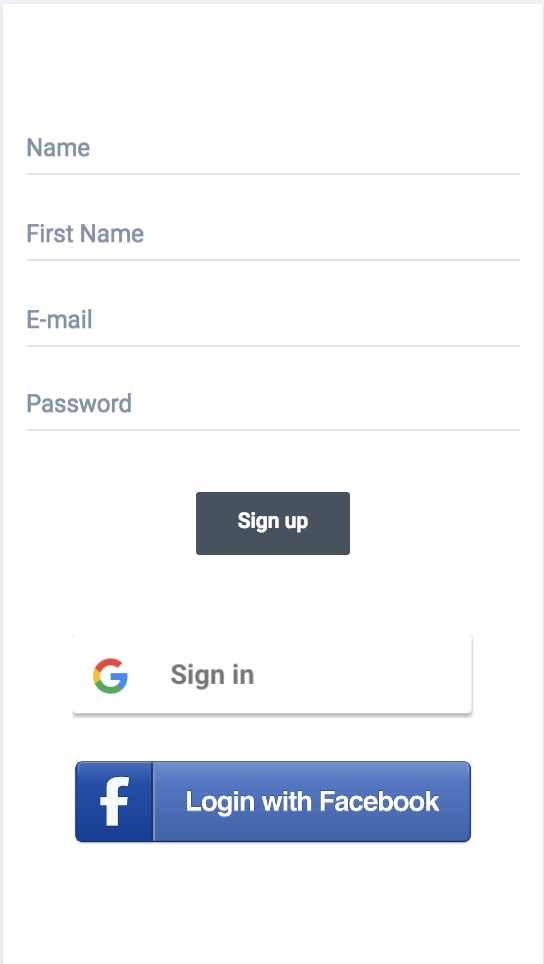
\includegraphics[scale=0.3]{ihms/inscription}
\centering
\hskip2em
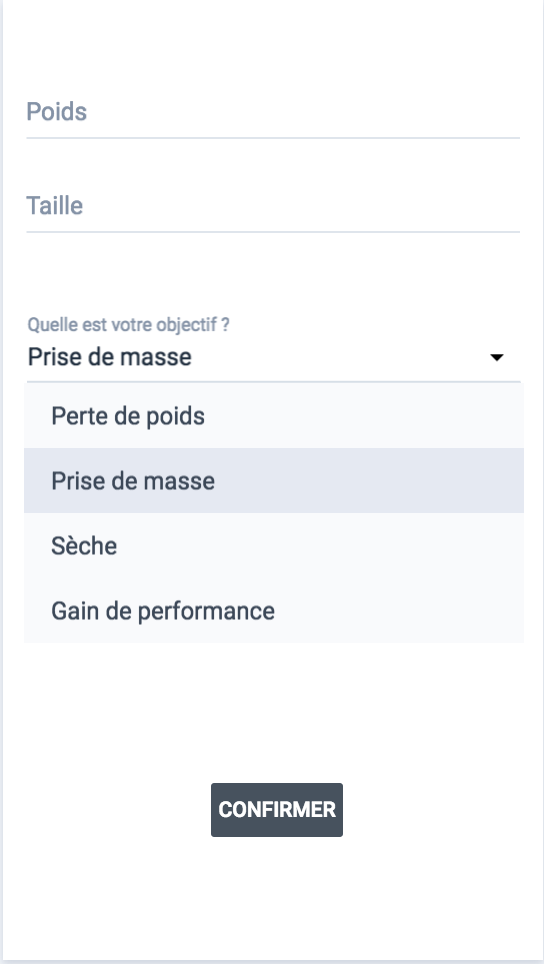
\includegraphics[scale=0.3]{ihms/caracteristiques}
\caption{Interfaces d'inscription}
\end{figure}


\begin{itshape}
User story : En tant qu'utilisateur, je veux rentrer mes données et caractéristiques personnelles dans le système pour m'inscrire.
\end{itshape}

\subsection{Didactitiel}

Lorsque le scénario d'inscription est terminé, une séance est générée automatiquement au client selon son type de sport choisi. L'application lui proposera de cliquer sur tous les boutons disponibles, étapes par étapes à l?aide d?indications afin de bien prendre en main l'application. Une fois la séance terminée, l'utilisateur reçoit un badge pour avoir effectuer sa toute première séance.\\


\begin{itshape}

User stories :

\begin{itemize}
\item En tant qu'utilisateur, je veux prendre l?application en main pour pouvoir l'utiliser à bon escient par la suite.
\item En tant que système, je propose un didacticiel à l'utilisateur pour que celui-ci utilise l'application correctement.
\end{itemize}

\end{itshape}

\subsection{Utilisation normale (en séance)}
L'utilisateur, avant de pouvoir générer une séance de sport, doit préciser le sport, l'intensité et le temps à consacrer pour sa séance. Le formulaire qu'il devra compléter sera pré-remplie en fonction des choix de ses séances précédentes.   

\begin{figure}[!h]
\centering
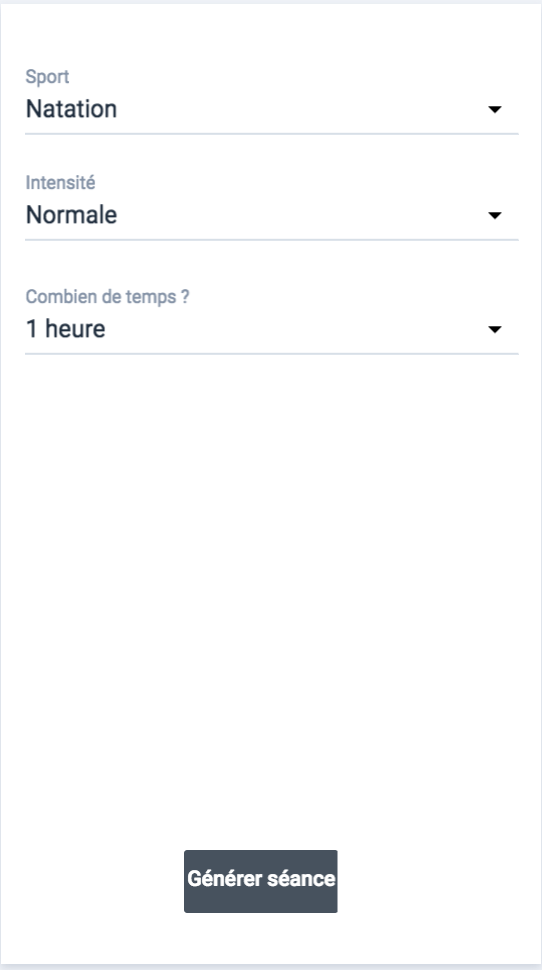
\includegraphics[scale=0.3]{ihms/seance}
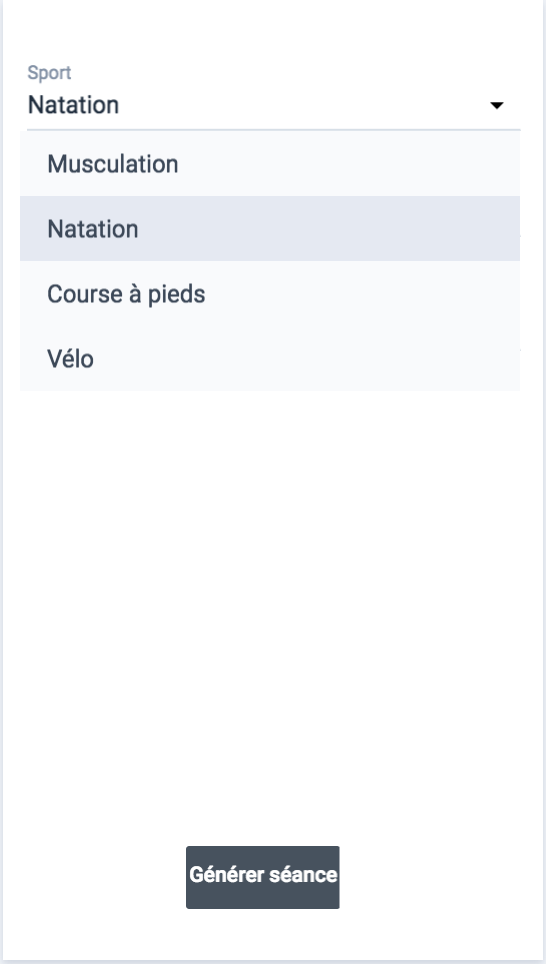
\includegraphics[scale=0.3]{ihms/seance2}
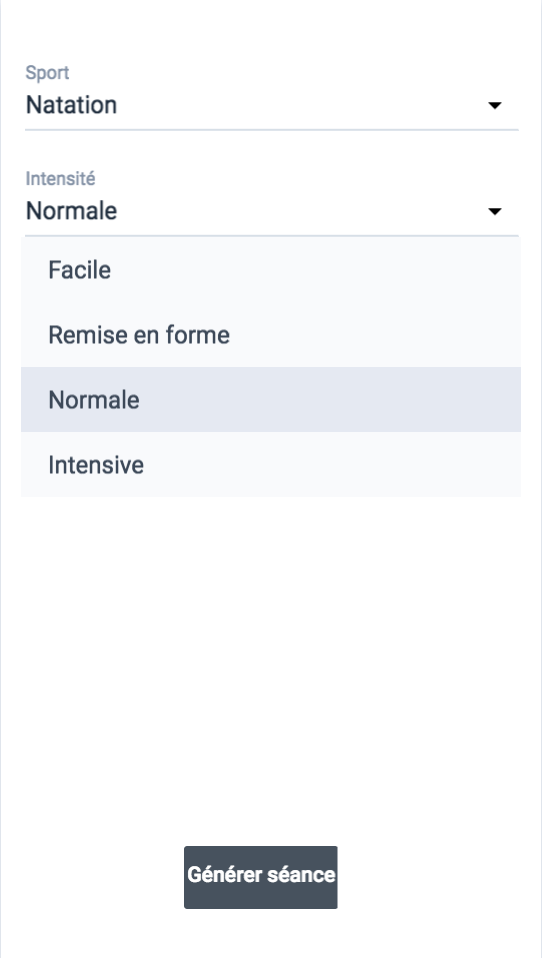
\includegraphics[scale=0.3]{ihms/seance3}
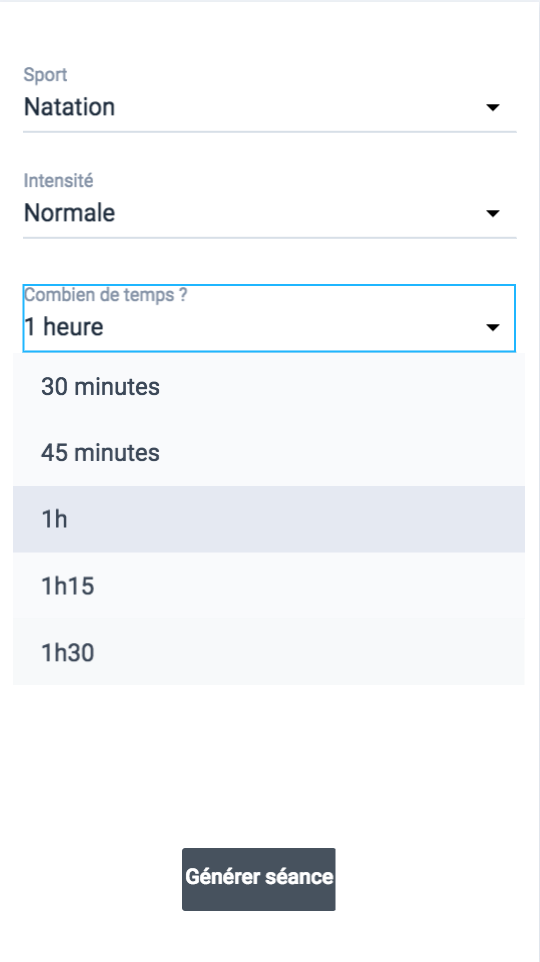
\includegraphics[scale=0.3]{ihms/seance4}
\caption{Interface de préparation de la séance}
\end{figure}

Une fois qu'il a confirmé ces informations, la séance est généré en fournissant à l'utilisateur une liste d'exercice à faire. Pour chaque exercice proposé, l'utilisateur pourra cliquer sur un sigle "Help" afin d'en savoir davantage sur l'exercice à réaliser. Ces informations d'aide peuvent être de types différents (vidéo, illustrations, texte). Une fois que l'utilisateur a fini tout les exercices, il doit valider sa séance en appuyant sur un bouton prévue à cette effet.\\ 

\begin{figure}[!h]
\centering
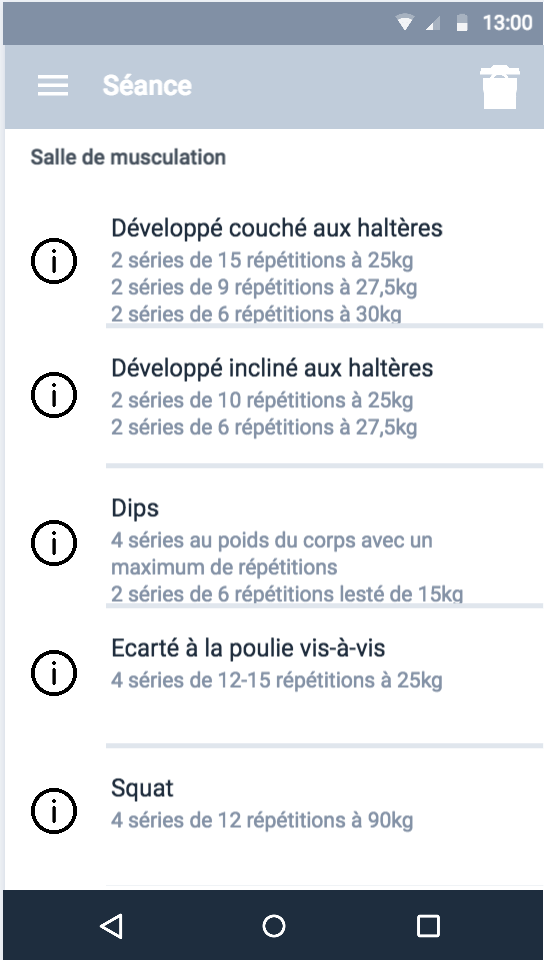
\includegraphics[scale=0.3]{ihms/normal_session}
\hskip2em
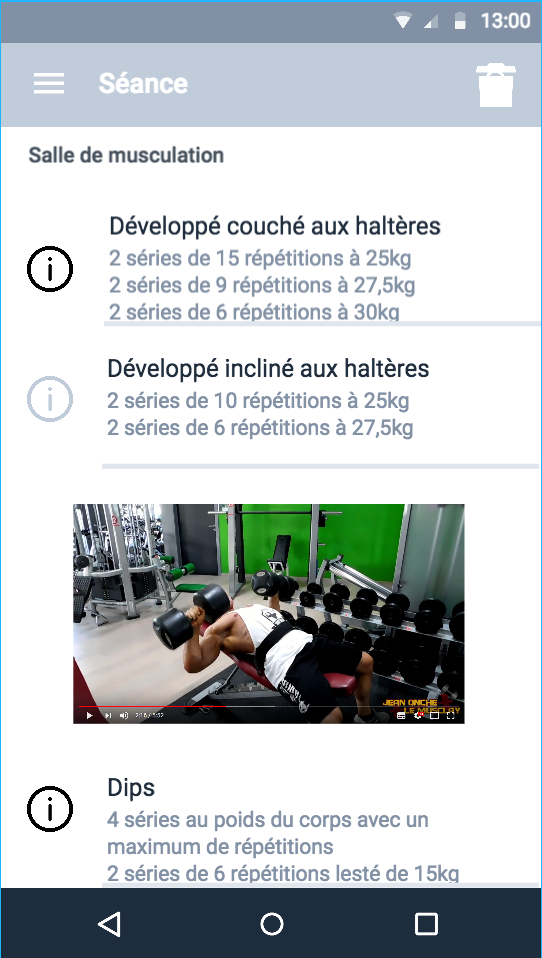
\includegraphics[scale=0.3]{ihms/get_information_about_exo}
\caption{Interface de la séance}
\end{figure}

\begin{itshape}
User story : En tant qu'utilisateur, j'attribue une cotation pour chacun des critères proposés pour améliorer le système dans sa globalité et le contenu des futures séances.

\end{itshape}

\subsection{Mise à jour des données (post-séance)}

Une fois la séance terminé et validé par l'utilisateur, les données d'entrainement sont mis à jour à l'aide de plusieurs critère tels que l'impression générale, la difficulté, ou si la durée de l'entrainement a été respecté. Chaque critère est côté sur base d'une note sur 5 donnée par l'utilisateur. Dès que l'utilisateur a validé toutes ses notes, il peut les confirmer et retourner sur l'écran d'accueil. L'application lui affiche un compteur de temps jusqu'à la prochaine séance "conseillé". L'utilisateur reçoit un badge toutes les 10 séances respectées et sa barre de progression est mis à jour.  

\begin{figure}[!h]
\centering
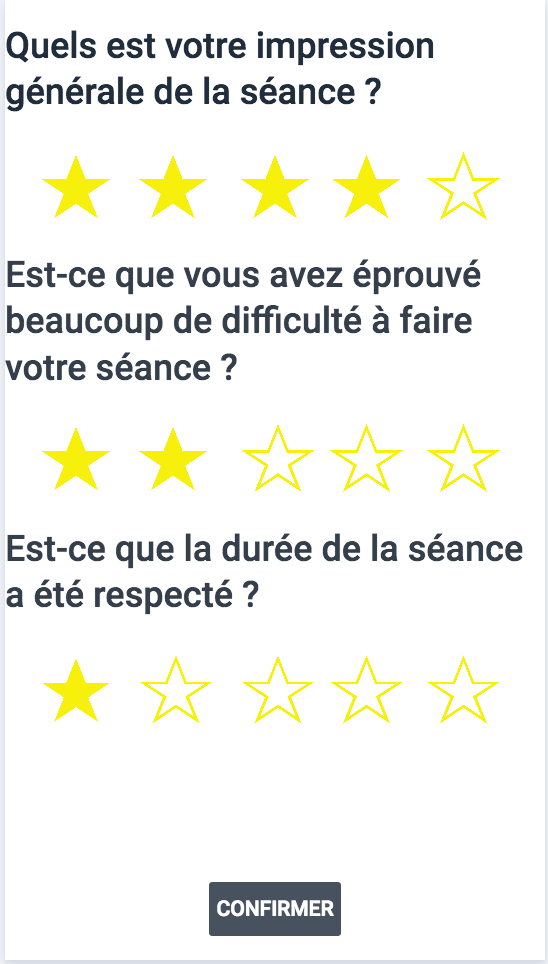
\includegraphics[scale=0.3]{ihms/rating_before_update}
\caption{Interface de mise à jour des données de post-séance}
\end{figure} 

\begin{itshape}
En tant qu'utilisateur, j'attribue une cotation pour chacun des critères proposés pour améliorer le système dans sa globalité et le contenu des futures séances.
\end{itshape}

\subsection{Suppression d'exercices d'une séance}

Lors de la génération de la séance, l'utilisateur peut cliquer sur une molette qui permettra de supprimer des exercices. Dans ce cas, une icône apparaît à côté de chaque exercice. Lorsqu'il clique dessus, il peut justifier son choix afin que l?exercice revienne dans les programmes dans plus ou moins longtemps.

\begin{figure}[!h]
\centering
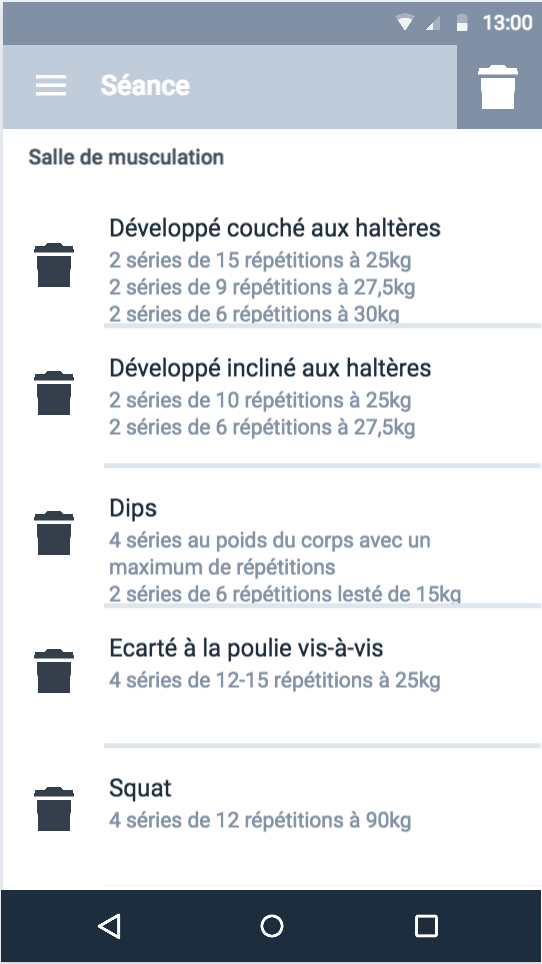
\includegraphics[scale=0.3]{ihms/remove_exo}
\caption{Suppression exercice}
\end{figure}

\begin{itshape}
User story : En tant qu'utilisateur, je choisis de supprimer des exercices inintéressants pour m'offrir une séance optimale et donner un feedback pour la suite de ces séances.
\end{itshape}

\subsection{Recherche d'un complexe sportif par un utilisateur}

L'utilisateur doit pouvoir sélectionner son sport, et selon sa localisation, l'application lui propose le complexe sportif adéquat à proximité. En cliquant dessus, quelques infos seront données, comme la fréquentation, le matériel mis à disposition?\\

\begin{itshape}
User story : En tant que système, je propose à l'utilisateur les complexes sportifs les plus proches correspondant aux exigences et à la localisation de celui-ci pour que l'utilisateur soit conseillé de la meilleure des manières.

\end{itshape}